\documentclass[11pt]{article}
\usepackage[letterpaper,margin=1in]{geometry}
\usepackage[T1]{fontenc}
\usepackage{mathptmx}
\usepackage[protrusion=true,expansion=true]{microtype}
\usepackage{amsmath,amssymb,amsthm,mathtools}
\usepackage{graphicx}
\usepackage{booktabs,array,tabularx}
\usepackage[table]{xcolor}
\usepackage{tikz}
\usetikzlibrary{arrows.meta,positioning,calc}
\usepackage[authoryear,round]{natbib}
\usepackage{enumitem}
\usepackage{wrapfig}
\usepackage[font=small,labelfont=bf,skip=4pt]{caption}
\usepackage{tcolorbox}
\usepackage{multicol}
\usepackage{titlesec}
\usepackage{needspace}
\titlespacing*{\section}{0pt}{2.4ex plus .8ex minus .3ex}{1.1ex plus .2ex}
\titlespacing*{\subsection}{0pt}{1.9ex plus .6ex minus .3ex}{0.8ex plus .2ex}
\titlespacing*{\paragraph}{0pt}{1.4ex plus .5ex minus .2ex}{0.8em}
\usepackage[colorlinks=true,linkcolor=blue!50!black,citecolor=blue!50!black,urlcolor=blue!50!black]{hyperref}
\usepackage[capitalise,nameinlink]{cleveref}

\setlength{\bibsep}{1.1pt}
\renewcommand{\bibfont}{\footnotesize}
\setlength{\parskip}{0pt}

\newcolumntype{Y}{>{\raggedright\arraybackslash}X}
\newcolumntype{L}[1]{>{\raggedright\arraybackslash}p{#1}}
\newtheorem{theorem}{Theorem}
\newtheorem{proposition}{Proposition}
\theoremstyle{remark}
\newtheorem*{remark}{Remark}

\newcommand{\QJ}{\textsc{qj}}
\newcommand{\ARZ}{\textsc{arz}}
\newcommand{\GO}{\textsc{go}}
\newcommand{\BJ}{\textsc{bj}}
\newcommand{\TV}{\mathrm{TV}}
\newcommand{\Gap}{\mathrm{Gap}}
\newcommand{\E}{\mathbb{E}}
\newcommand{\X}{\mathcal{X}}
\newcommand{\tmix}{t_{\mathrm{mix}}}
\newcommand{\DG}{\mathrm{DG}}
\newcommand{\RG}{\mathrm{RG}}
\newcommand{\RC}{\mathrm{RC}}
\newcommand{\DC}{\mathrm{DC}}

\title{\vspace{-1.2cm}\textbf{Exact Draws, Approximate Draws:}\\[2pt]
\Large A Survey of Convergence Theory for Gibbs and Metropolis-within-Gibbs Samplers}
\author{Preet Shah}
\date{November 2026}

\begin{document}
\maketitle

\begin{abstract}
\noindent Markov chain Monte Carlo (MCMC) algorithms are randomized algorithms whose correctness is easy to certify but whose running time is notoriously hard to bound: a chain can have exactly the right stationary distribution and still need an enormous number of steps to forget its starting point. This survey explains how the speed of two workhorse methods, the Gibbs sampler and its practical relative Metropolis-within-Gibbs, is analyzed, and places four recent papers within seven decades of work on MCMC convergence. We organize the material around a \emph{decomposition principle}: a Metropolis-within-Gibbs sampler is as fast as the idealized Gibbs sampler it imitates, whose speed reflects the dependence structure of the target, degraded by the quality of the local Metropolis--Hastings moves that replace exact conditional draws. \citet{qin2022convergence} make this exact for two components through the geometry of projections; \citet{ascolani2026scalability} make it quantitative and dimension-free through conditional conductance; \citet{brown2024convergence} describe what controls the local factor; and \citet{gerencser2023rates} pin down the global factor for a model of almost exchangeable data, proving a $\Theta(A^2)$ mixing time by coupling. Simulations illustrate the main phenomena, and we close with open problems.
\end{abstract}

%======================================================================
\section{Introduction}\label{sec:intro}

Suppose we want samples from a distribution $\pi$ on a high-dimensional space $\X$ whose density is known only up to a normalizing constant, as for a Bayesian posterior or a Boltzmann distribution. Markov chain Monte Carlo (MCMC) is a randomized algorithm for this task: design a Markov chain with stationary distribution $\pi$, run it for $t$ steps, and output the final state. Proving that the law of the output converges to $\pi$ is usually easy, because it reduces to a local balance equation. Proving that it converges \emph{quickly}, so that $t$ stays modest as the problem grows, is hard, and it is the subject of this survey.

The gap between ``correct'' and ``fast'' is not a technicality. \Cref{fig:geometry}(b) shows the Gibbs sampler, which redraws one coordinate at a time from its conditional distribution, on a bivariate Gaussian with correlation $0.95$. Every move is an exact conditional draw, so the chain is provably correct; but the mass lies on a thin diagonal ridge and the sampler moves only parallel to the axes, so it creeps along in short steps. With correlation $\rho$ the error shrinks by only $\rho^2$ per sweep (\cref{sec:running}), so about $1/(1-\rho^2)$ sweeps are needed. In models with thousands of parameters, similar ridges arise from dependence that no one can visualize, and the slowdown can be severe yet invisible in the output.

\begin{figure}[t]
\centering
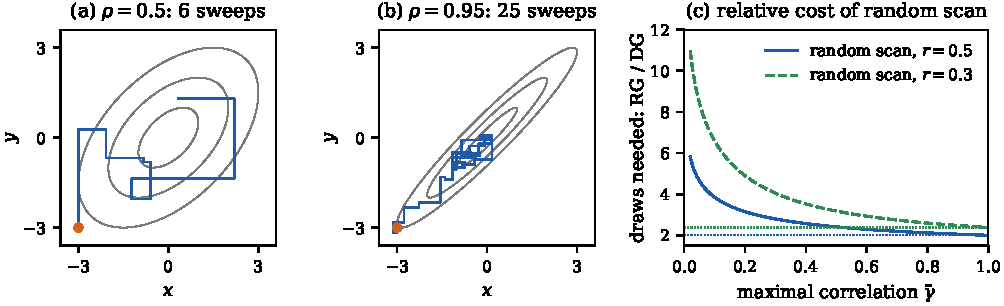
\includegraphics[width=\textwidth]{figs/fig_gibbs_geometry.pdf}
\caption{Gibbs sampling a standard bivariate Gaussian. (a,~b)~Deterministic-scan paths from the same start (orange); contours at 1, 2, 3 standard deviations. Under strong correlation the axis-parallel moves are short relative to the ridge. (c)~Cost of randomizing the scan implied by \cref{thm:qj}: conditional draws a random scan with selection probability $r$ needs per draw of the deterministic scan, versus the maximal correlation $\bar\gamma$; dotted lines mark the limits $1/(2r(1-r))$.}
\label{fig:geometry}
\end{figure}

\paragraph{A large and old field.} MCMC convergence has been studied for over seventy years by two communities. Probabilists and statisticians built the theory of general state-space chains, with criteria for geometric convergence and explicit drift-and-minorization bounds \citep{meyn2009,rosenthal1995}; theoretical computer scientists, seeking polynomial-time algorithms for counting and volume computation, built conductance and coupling arguments \citep{sinclair1989,dyer1991volume,jerrum2004permanent}. \Cref{sec:history} surveys both. Recently the traditions have converged on \emph{quantitative} bounds that show how running time depends on dimension and sample size, for the algorithms practitioners actually run.

\paragraph{Focus: ideal versus implementable updates.} Practitioners rarely run the pure Gibbs sampler, because exact conditional draws exist only for conditionally conjugate models. They replace each draw by one or a few Metropolis--Hastings steps that leave the conditional invariant, producing a \emph{Metropolis-within-Gibbs} (MwG) sampler, whose theory is still young. The four papers surveyed here attack this gap from complementary directions and support one organizing idea, the \emph{decomposition principle}:
\begin{equation}\label{eq:principle}
\underbrace{\text{speed of Metropolis-within-Gibbs}}_{\text{what we run}}\;\approx\;\underbrace{\text{speed of exact Gibbs}}_{\text{global: dependence in }\pi}\;\times\;\underbrace{\text{quality of the conditional updates}}_{\text{local: tuning, block dimension}}.
\end{equation}
\citet[henceforth \QJ]{qin2022convergence} make~\eqref{eq:principle} exact for two components, using that exact Gibbs updates are orthogonal projections. \citet[\ARZ]{ascolani2026scalability} prove a quantitative version for many components, in terms of conductance, and show that MwG for high-dimensional hierarchical models mixes in a number of iterations that does not grow with the dimension. \citet[\BJ]{brown2024convergence} review what controls Metropolis--Hastings convergence, and their lower bounds \citep{brown2024lower} explain when the local factor collapses. \citet[\GO]{gerencser2023rates} compute the global factor for a Gibbs sampler used with almost exchangeable data, proving matching bounds of order $A^2$ by coupling. \Cref{fig:map} shows how the pieces fit.

\begin{figure}[t]
\centering
\begin{tikzpicture}[
  box/.style={draw=black!50, rounded corners=3pt, align=left, inner sep=4.5pt, minimum width=7.4cm, fill=#1, font=\footnotesize},
  arr/.style={-{Stealth[length=2.6mm]}, thick, black!65}]
\node[box=blue!5, text width=7.1cm, anchor=south west] (G) at (0,0.22) {\textbf{Global factor: the exact Gibbs sampler $G$}\\ set by dependence in $\pi$ (maximal correlation, ridges)\\[2pt] \GO\ (\S\ref{sec:go}): explicit $\Theta(A^2)$ rate for de Finetti's prior\\ \QJ\ (\S\ref{sec:gibbs}): deterministic vs.\ random scan, exactly};
\node[box=orange!8, text width=7.1cm, anchor=north west] (L) at (0,-0.22) {\textbf{Local factor: conditional MH updates}\\ how close each block move is to an exact draw\\[2pt] \BJ\ (\S\ref{sec:mh}): acceptance, tuning in $d$ and $n$, lower bounds;\\ independence vs.\ random-walk proposals};
\node[box=green!7, text width=7.1cm, anchor=west] (P) at (8.75,0) {\textbf{What we run: Metropolis-within-Gibbs $P$} (\S\ref{sec:mwg})\\[2pt] \QJ\ (two blocks, $L^2$): MH cannot beat the barrier $\bar\gamma$;\\ when Gibbs and hybrids are geometrically ergodic\\[2pt] \ARZ\ (many blocks, conductance):\\ $\kappa\,\Phi_s(G)-\pi(K^c)/s\;\le\;\Phi_s(P)\;\le\;\Phi_s(G)$;\\ dimension-free mixing for hierarchical models};
\draw[arr] (G.east) -- (P.north west);
\draw[arr] (L.east) -- (P.south west);
\node[font=\Large] at (8.05,0) {$\times$};
\end{tikzpicture}
\caption{Map of the survey: the four papers supply the two factors of the decomposition principle~\eqref{eq:principle} and the theorems that combine them.}
\label{fig:map}
\end{figure}

\paragraph{Roadmap.} \Cref{sec:prelim} fixes notation and the basic quantities, and \cref{sec:history} reviews the classical toolbox. \Cref{sec:gibbs,sec:go,sec:mh} study the two factors of~\eqref{eq:principle} separately (\QJ, \GO, \BJ), \cref{sec:mwg} combines them (\QJ, \ARZ), \cref{sec:synthesis} compares the papers, and \cref{sec:open} lists open problems. We give proofs only when they are short and illuminating, and otherwise describe proof architectures.

%======================================================================
\section{Preliminaries: Markov chains as randomized algorithms}\label{sec:prelim}

\subsection{Kernels, stationarity, and three algorithms}
A Markov chain on $\X$ is specified by a transition kernel $P(x,\cdot)$, the law of the next state given the current state $x$; from an initial law $\mu$, the state after $t$ steps has law $\mu P^t$. A distribution $\pi$ is \emph{stationary} if $\pi P=\pi$, and $P$ is \emph{reversible} if $\pi(dx)P(x,dy)=\pi(dy)P(y,dx)$ (detailed balance), which implies stationarity. Under mild irreducibility and aperiodicity conditions $\mu P^t\to\pi$ from every start \citep{tierney1994,roberts2004general}: correctness is cheap.

We split $x=(x_1,\dots,x_d)$ into blocks, write $x_{-i}$ for all blocks but the $i$th, and $\pi_i(\cdot\mid x_{-i})$ for the conditional law of block $i$. \Cref{fig:alg} defines the algorithms. Each Metropolis--Hastings (MH) step is reversible with respect to its target \citep{metropolis1953,hastings1970}, as is each exact Gibbs update and any random-scan mixture of reversible updates; a deterministic scan is a product of updates and usually \emph{not} reversible, one reason it is harder to analyze.

\begin{figure}[t]
\begin{tcolorbox}[colback=gray!3,colframe=gray!45,boxrule=0.4pt,left=5pt,right=5pt,top=3pt,bottom=3pt,arc=2pt]
\small
\textbf{One step of a component-wise sampler} from the state $x=(x_1,\dots,x_d)$:
\begin{enumerate}[leftmargin=1.4em,nosep]
\item \emph{Choose a block.} Random scan: draw $i\in\{1,\dots,d\}$ with probabilities $r_1,\dots,r_d$ (often uniform). Deterministic scan: visit $i=1,2,\dots,d$ in order; one pass is a \emph{sweep}.
\item \emph{Update block $i$}, leaving $x_{-i}$ unchanged.
\textbf{Gibbs:} draw $x_i'\sim\pi_i(\cdot\mid x_{-i})$ exactly.
\textbf{Metropolis-within-Gibbs:} propose $y\sim q_i(x_i,\cdot)$ and set $x_i'=y$ with probability
$\alpha_i=\min\Bigl\{1,\frac{\pi_i(y\mid x_{-i})\,q_i(y,x_i)}{\pi_i(x_i\mid x_{-i})\,q_i(x_i,y)}\Bigr\}$, otherwise $x_i'=x_i$.
\end{enumerate}
Plain Metropolis--Hastings is the case of one block. Common proposals: random walk $N(x,hI)$; independence $q(x,\cdot)=q(\cdot)$; MALA $N\bigl(x+\tfrac h2\nabla\log\pi(x),hI\bigr)$.
\end{tcolorbox}
\vspace{-6pt}
\caption{The algorithms studied in this survey.}
\label{fig:alg}
\end{figure}

\subsection{How close is close? Distances and mixing times}
We measure the distance to $\pi$ in three ways. \emph{Total variation}, $\|\mu-\nu\|_\TV=\sup_A|\mu(A)-\nu(A)|$, bounds the error in the probability of any event. The \emph{Wasserstein} distance $W(\mu,\nu)=\inf\E[\mathrm{dist}(X,Y)]$ over couplings of $X\sim\mu$ and $Y\sim\nu$ bounds the error of every 1-Lipschitz statistic and is often better behaved in high dimension. The \emph{$\chi^2$ (or $L^2$)} distance $\|d\mu/d\pi-1\|_{L^2(\pi)}$ is the strongest and the most convenient for spectral arguments, since $\|\mu-\pi\|_\TV\le\frac12\|d\mu/d\pi-1\|_{L^2(\pi)}$.

The \emph{mixing time} $\tmix(\varepsilon;\mu)=\min\{t:\mathrm{dist}(\mu P^t,\pi)\le\varepsilon\}$ is the algorithm's running time, studied from a worst-case start or from an \emph{$M$-warm start} ($\mu(A)\le M\pi(A)$ for all $A$), which removes the cost of locating the bulk of $\pi$. Statisticians often study \emph{geometric ergodicity} instead, $\|P^t(x,\cdot)-\pi\|_\TV\le C(x)\rho^t$ with $\rho<1$ (\emph{uniform} ergodicity if $C$ is bounded). It guarantees central limit theorems for MCMC averages but is qualitative: it says nothing about how close $\rho$ is to $1$, which determines the running time.

\subsection{The operator view: spectral gaps, conductance, and projections}\label{sec:operator}
A kernel acts on functions by $Pf(x)=\int f(y)P(x,dy)=\E[f(X_{t+1})\mid X_t=x]$. On $L^2(\pi)$ with inner product $\langle f,g\rangle_\pi=\int fg\,d\pi$, reversibility is exactly self-adjointness, and stationarity means $P$ preserves the subspace $L_0^2(\pi)$ of mean-zero functions. The \emph{$L^2$ convergence rate} $\rho(P)$ is the smallest $\rho$ with $\|\mu P^t-\pi\|_{L^2}\le C_\mu\rho^t$ for all $\mu$ with $d\mu/d\pi\in L^2(\pi)$; for reversible $P$ it is the operator norm $\|P\|_{L^2_0(\pi)}$, and $\rho(P)<1$ is equivalent to geometric ergodicity \citep{roberts1997geometric}. A reversible chain from an $M$-warm start therefore satisfies
\begin{equation}\label{eq:L2mix}
\|\mu P^t-\pi\|_\TV\le\tfrac12\sqrt{M-1}\;\rho(P)^t,\qquad\text{so}\qquad \tmix(\varepsilon)\le\frac{\log\bigl(\sqrt{M}/(2\varepsilon)\bigr)}{1-\rho(P)}.
\end{equation}
The \emph{spectral gap} is $\Gap(P)=\inf_f\mathcal E_P(f)/\mathrm{Var}_\pi(f)$, where the \emph{Dirichlet form} $\mathcal E_P(f)=\langle f,(I-P)f\rangle_\pi=\frac12\iint(f(y)-f(x))^2\,\pi(dx)P(x,dy)$ measures how much $P$ moves $f$; it equals $1-\rho(P)$ when $P$ has no negative spectrum (e.g., for lazy chains).

Spectral quantities are hard to compute directly. The \emph{conductance}
\[
\Phi(P)=\inf_{0<\pi(A)\le1/2}\frac{P(\partial A)}{\pi(A)},\qquad P(\partial A)=\int_A P(x,A^c)\,\pi(dx),
\]
measures the worst bottleneck: $P(\partial A)/\pi(A)$ is the chance of leaving $A$ in one step from $\pi$ restricted to $A$. Cheeger's inequality for reversible chains \citep{lawler1988,sinclair1989} brackets the gap by conductance,
\begin{equation}\label{eq:cheeger}
\tfrac12\,\Phi(P)^2\;\le\;\Gap(P)\;\le\;2\,\Phi(P).
\end{equation}
The \emph{$s$-conductance} $\Phi_s(P)$ takes the infimum only over sets with $s<\pi(A)\le\frac12$ \citep{lovasz1993random}; ignoring small sets costs only an additive error from a warm start (under mild conditions such as laziness):
\begin{equation}\label{eq:sconductance}
\|\mu P^t-\pi\|_\TV\le Ms+M\bigl(1-\tfrac12\Phi_s(P)^2\bigr)^t\qquad\text{for every $M$-warm }\mu.
\end{equation}
This flexibility will be crucial in \cref{sec:arz}.

\paragraph{Gibbs updates are projections.} The observation behind much of \cref{sec:gibbs} is that the exact Gibbs update of block $i$ acts on functions by
\[
G_if(x)=\int f(x_{-i},y)\,\pi_i(dy\mid x_{-i})=\E_\pi\bigl[f(X)\bigm| X_{-i}=x_{-i}\bigr],
\]
and conditional expectation is the \emph{orthogonal projection} of $L^2(\pi)$ onto the subspace of functions not depending on $x_i$. Thus $G_i^2=G_i$; a deterministic-scan Gibbs sampler is a product of projections (von Neumann's method of alternating projections, run with random inputs), and a random-scan Gibbs sampler is a convex combination of projections. Its Dirichlet form is the average conditional variance, $\mathcal E_{G_i}(f)=\E_\pi[\mathrm{Var}_\pi(f(X)\mid X_{-i})]$.

\subsection{Running example: the bivariate Gaussian}\label{sec:running}
Let $(X,Y)$ be standard bivariate Gaussian with correlation $\rho$, so $X\mid Y=y\sim N(\rho y,1-\rho^2)$ and symmetrically. One deterministic sweep (update $Y$, then $X$) gives $X'=\rho^2X+\sqrt{1-\rho^4}\,\xi$ with $\xi\sim N(0,1)$, an autoregression whose memory decays like $\rho^{2t}$: the rate is $\rho^2$ per sweep, and reducing the error by a constant factor takes about $1/(1-\rho^2)$ sweeps when $\rho$ is near $1$. Geometrically (\cref{fig:geometry}a,b), the mass lies on a ridge of length of order one and width of order $\sqrt{1-\rho^2}$, each axis-parallel move is about as long as the ridge is wide, and the number of sweeps scales like $(\text{length}/\text{width})^2$. We will meet this \emph{aspect-ratio-squared} heuristic again in \cref{sec:go}, where the ridge is the diagonal of a cube.

%======================================================================
\section{Seventy years of convergence analysis}\label{sec:history}

\subsection{From physics to statistics}
The Metropolis algorithm was invented to compute equilibrium properties of interacting particles \citep{metropolis1953}; \citet{hastings1970} generalized it to asymmetric proposals. \citet{geman1984} introduced the Gibbs sampler for Bayesian image restoration, and \citet{gelfand1990} showed statisticians that it could compute posteriors in otherwise intractable models, launching what \citet{diaconis2009revolution} called the MCMC revolution. The theory of the 1990s settled the qualitative questions first. \citet{tierney1994} gave general conditions for convergence and central limit theorems; \citet{mengersen1996} showed that the independence sampler is uniformly ergodic exactly when the target-to-proposal density ratio is bounded, and that random-walk Metropolis is geometrically ergodic essentially when the target has exponentially light tails, a theory \citet{roberts1996geometric} and \citet{jarner2000} extended to many dimensions. For Gibbs samplers, \citet{liu1994covariance} tied convergence to correlation structure, \citet{amit1991} and \citet{roberts1997updating} analyzed Gaussian targets, and \citet{roberts1997geometric} began the theory of hybrid samplers.

\subsection{The classical toolbox}
\Cref{tab:toolbox} summarizes the main techniques; each surveyed paper uses at least one, and part of our aim is to explain why each chose the tool it did.

\emph{Drift and minorization.} A minorization condition $P(x,\cdot)\ge\epsilon\,\nu(\cdot)$ for $x$ in a ``small'' set $C$ lets the chain regenerate with probability $\epsilon$ from anywhere in $C$; a drift condition $PV\le\lambda V+b$ ($\lambda<1$) says a Lyapunov function $V$ pulls the chain back toward $C$. Coupling two copies that regenerate together yields explicit total-variation bounds \citep{rosenthal1995}. This is the standard route to geometric ergodicity on general state spaces, but the constants degrade badly with dimension \citep{qin2021limitations,qin2022wasserstein}, and \GO\ note that it gives bounds exponentially bad in their concentration parameter.

\emph{Spectral methods and comparison.} Exact spectra give sharp answers when computable, as for a family of two-component Gibbs samplers analyzed with orthogonal polynomials \citep{diaconis2008gibbs}. More often one bounds the gap through its variational formula, by canonical paths \citep{diaconis1991geometric} or by \emph{comparison}: if $\mathcal E_P(f)\ge c\,\mathcal E_Q(f)$ for all $f$ and both chains share $\pi$, then $\Gap(P)\ge c\,\Gap(Q)$ \citep{diaconis1993comparison}. Comparison is the prototype of~\eqref{eq:principle}.

\emph{Conductance and isoperimetry.} Cheeger's inequality~\eqref{eq:cheeger} reduces mixing to showing that every set of moderate probability leaks mass. This idea underlies polynomial-time algorithms for the permanent \citep{sinclair1989,jerrum2004permanent} and for convex-body volume \citep{dyer1991volume,lovasz1993random}, and recently gave the first explicit spectral-gap bounds for random-walk Metropolis on $\mathbb R^d$ \citep{andrieu2024explicit}. Decomposition theorems bound a chain's gap through pieces of it \citep{madras2002}.

\emph{Coupling and Wasserstein contraction.} If two copies can be coupled so that their distance contracts on average by a factor $1-c$ per step, then $W(\mu P^t,\pi)\le(1-c)^tW(\mu,\pi)$. Path coupling \citep{bubley1997path} made this routine for discrete systems, and monotone couplings power exact sampling \citep{propp1996exact}. In continuous spaces, Wasserstein versions of Harris's theorem and of drift arguments \citep{hairer2011asymptotic,durmus2015quantitative,qin2022wasserstein} avoid the dimension penalty of minorization.

\emph{Scaling limits and asymptotics.} For product-form targets in dimension $d$, random-walk Metropolis must use proposal variance of order $1/d$ (acceptance rate near $0.234$) and then needs order $d$ steps \citep{roberts1997weak}; the Metropolis-adjusted Langevin algorithm (MALA) needs variance of order $d^{-1/3}$ \citep{roberts1998optimal}. Such diffusion limits identify the right scaling, and non-asymptotic bounds under log-concavity now exist \citep{dwivedi2019}. Posterior concentration as the sample size grows can also make MCMC analysis tractable \citep{belloni2009}; it is central to \ARZ.

\emph{Lower bounds} certify that an algorithm is slow, which matters as much in practice as proving it fast. They come from slowly moving test functions, from bottleneck sets, and, for accept--reject algorithms, from the probability of not moving at all \citep{brown2024lower}.

\begin{table}[t]
\centering\footnotesize
\renewcommand{\arraystretch}{1.18}
\begin{tabularx}{\textwidth}{@{}L{2.15cm}YYYL{2.75cm}@{}}
\toprule
\textbf{Technique} & \textbf{What one shows} & \textbf{Strengths} & \textbf{Weaknesses} & \textbf{Representative work} \\
\midrule
Drift \& minorization & $PV\le\lambda V+b$; \ $P(x,\cdot)\ge\epsilon\nu$ on $\{V\le R\}$ & General state spaces; explicit TV bounds; standard route to geometric ergodicity & Constants degrade fast with dimension; blind to diffusive behavior & \citet{rosenthal1995}; \citet{meyn2009}; \citet{qin2021limitations} \\
Spectral \& comparison & bound $\inf\mathcal E_P(f)/\mathrm{Var}(f)$, or $\mathcal E_P\ge c\,\mathcal E_Q$ & Sharp when spectra are computable; transfers bounds between chains & Needs reversibility; exact spectra rare & \citet{diaconis1993comparison}; \citet{liu1994covariance}; \QJ \\
Conductance \& isoperimetry & every set leaks: $P(\partial A)\ge\Phi\,\pi(A)$ & Geometric and robust; $s$-version ignores rare bad sets & Squaring loss in~\eqref{eq:cheeger}; needs isoperimetry of $\pi$ & \citet{sinclair1989}; \citet{lovasz1993random}; \ARZ \\
Coupling \& Wasserstein & two copies contract on average & Scales well with dimension; natural for monotone or contractive dynamics & Couplings are model-specific; TV needs extra work & \citet{bubley1997path}; \citet{qin2022wasserstein}; \GO \\
Scaling limits \& asymptotics & diffusion limits; posterior concentration & Identifies the right tuning and scaling & Asymptotic; restricted model classes & \citet{roberts1997weak}; \citet{belloni2009}; \ARZ \\
Lower bounds & slow test functions; holding probabilities & Certify failure; guide tuning & Rarely matched by upper bounds & \citet{brown2024lower}; \GO \\
\bottomrule
\end{tabularx}
\caption{The classical toolbox for MCMC convergence, and where the surveyed papers use it.}
\label{tab:toolbox}
\end{table}

\subsection{The modern agenda}
Two developments shape current research. The first is \emph{convergence complexity}: how mixing times scale as the dimension $p$ and sample size $n$ grow \citep{rajaratnam2015,qin2019convergence}. A recurring surprise is that well-designed Gibbs samplers can be \emph{dimension-free}, mixing in a number of iterations bounded independently of the dimension \citep{jin2022dimension,ascolani2024dimension}, whereas gradient-based methods pay polynomial factors. The second is the analysis of \emph{hybrid} samplers. Early results were qualitative, transferring uniform or geometric ergodicity between scans and between Gibbs and MwG under conditions \citep{roberts1997geometric,fort2003,jones2014conditional}; \QJ, \ARZ, and the concurrent spectral analysis of \citet{qin2025spectral} made the relationship sharp or quantitative. In terms of \cref{tab:toolbox}, \QJ\ use spectral geometry and kernel comparison, \ARZ\ conductance plus Bayesian asymptotics, \GO\ Wasserstein coupling plus test-function lower bounds, and \BJ\ survey drift, spectral, and Wasserstein methods for MH with an emphasis on lower bounds.

%======================================================================
\section{The geometry of exact Gibbs sampling}\label{sec:gibbs}

\subsection{Two blocks, two subspaces}
Let $\Pi$ be a joint law of $(X,Y)$ and consider the deterministic scan (DG), which draws $Y\mid X$ and then $X\mid Y$, and the random scan (RG), which updates $X$ with probability $r$ and $Y$ otherwise. Two-block samplers matter more than they appear to: every data-augmentation algorithm is one, and so is the alternation between global and local parameters in a hierarchical model (\cref{sec:hier}).

By \cref{sec:operator} the two updates are orthogonal projections in $L_0^2(\Pi)$: drawing a fresh $X$ projects a function onto the subspace $\mathcal H_Y$ of functions of $y$ alone, and drawing a fresh $Y$ projects onto the subspace $\mathcal H_X$ of functions of $x$ alone. The geometry of two subspaces is captured by the angle between them, whose cosine here is the \emph{maximal correlation}
\[
\bar\gamma=\sup\bigl\{\mathrm{Corr}\bigl(g(X),h(Y)\bigr):\ g,h\ \text{non-constant with finite variance}\bigr\}\in[0,1].
\]
For a Gaussian pair $\bar\gamma=|\rho|$. If $\bar\gamma=1$, some nontrivial functions of $X$ can be predicted arbitrarily well from $Y$, and no Gibbs sampler on these blocks converges geometrically. A classical result gives the deterministic-scan rate $\rho(P_\DG)=\bar\gamma^2$ \citep{liu1994covariance}: once a function depends on a single block, each half-sweep maps it to a function of the other block and shrinks it by at most the cosine $\bar\gamma$. What about the random scan, which is reversible and so easier to analyze, but wastes moves by sometimes repeating a block?

\begin{theorem}[\QJ]\label{thm:qj}
For every selection probability $r\in(0,1)$,
\[
\rho(P_\RG)=\frac{1+\sqrt{1-4r(1-r)\,\bigl(1-\rho(P_\DG)\bigr)}}{2},\qquad\text{where }\ \rho(P_\DG)=\bar\gamma^2.
\]
\end{theorem}

\subsection{Why the formula holds: two lines in a plane}
The formula looks mysterious, but it is a statement about two projections, and the smallest case contains the whole calculation. Suppose the relevant part of $L_0^2(\Pi)$ were a plane, with $\mathcal H_X$ spanned by a unit vector $u$ and $\mathcal H_Y$ by a unit vector $v$, so that $\langle u,v\rangle=\cos\theta=\bar\gamma$. The two updates are then the rank-one projections $uu^\top$ and $vv^\top$, and:
\begin{itemize}[leftmargin=1.3em,nosep]
\item a deterministic sweep acts as $uu^\top vv^\top=\cos\theta\,uv^\top$, whose only nonzero eigenvalue is $\cos^2\theta=\bar\gamma^2$;
\item a random-scan step acts as $R=r\,vv^\top+(1-r)\,uu^\top$, a symmetric $2\times2$ matrix with $\mathrm{tr}\,R=1$ and $\det R=r(1-r)\sin^2\theta$ (the product of the weights times the squared area spanned by $u$ and $v$). Its eigenvalues solve $\lambda^2-\lambda+r(1-r)(1-\bar\gamma^2)=0$, and the larger one is exactly the formula in \cref{thm:qj}.
\end{itemize}
In general, the theory of two projections \citep{bottcher2010gentle} splits the Hilbert space into pieces on which the pair looks like this planar picture at various angles, plus degenerate pieces on which the random scan has eigenvalue $0$, $r$, or $1-r$; both rates are set by the smallest angle, whose cosine is $\bar\gamma$. \QJ\ give a self-contained proof that avoids this machinery: $P_\RG f$ always has the form $g(x)+h(y)$, and on such sums the operator acts through a $2\times2$ structure,
\[
P_\RG(g\oplus h)=\bigl[(1-r)g+(1-r)Q_1h\bigr]\oplus\bigl[r\,Q_2g+r\,h\bigr],
\]
where $Q_1h(x)=\E[h(Y)\mid X=x]$ and $Q_2g(y)=\E[g(X)\mid Y=y]$.
Working with approximate eigenfunctions of the marginal chain $Q_1Q_2$, whose norm is $\bar\gamma^2$, and eliminating $h$ yields the same quadratic, $\bigl(\lambda-(1-r)\bigr)(\lambda-r)=r(1-r)\bar\gamma^2$.

\subsection{Consequences}
Several facts follow at once. The right side of \cref{thm:qj} is at least $\max\{r,1-r\}\ge\frac12$, so a random scan never contracts faster than $\frac12$ per step. The two rates are monotone functions of each other, so DG is geometrically ergodic if and only if RG is. The best selection probability is $r=\frac12$, giving $\rho(P_\RG)=(1+\bar\gamma)/2$. Most importantly, the deterministic scan is faster even after accounting for cost: a DG iteration makes two conditional draws and an RG iteration one, yet \QJ\ prove that DG wins when both run for the same computing time. \Cref{fig:geometry}(c) quantifies this. Counting conditional draws, the random scan needs at least $1/(2r(1-r))\ge2$ times as many draws as the deterministic scan to achieve the same contraction, and in the hard regime $\bar\gamma\to1$ the ratio tends to exactly $1/(2r(1-r))$, because $1-\rho(P_\RG)\approx r(1-r)(1-\bar\gamma^2)$ while the per-draw rate of DG satisfies $1-\bar\gamma\approx\frac12(1-\bar\gamma^2)$. In words: for two blocks, randomizing the scan order costs at least a factor of two in conditional draws, and with the best choice $r=\frac12$ the factor tends to exactly two as the problem gets hard.

\subsection{Beyond two blocks}
The planar picture is special to two subspaces. With three or more blocks the deterministic scan has no reversible marginal chains and the technique of \QJ\ does not extend; for many components the comparison between scans can go either way \citep{roberts2016surprising}, and \citet{andrieu2016random} compares scans through asymptotic variances instead. For Gaussian targets with any number of blocks, deterministic-scan Gibbs is a randomized Gauss--Seidel iteration whose rate is the spectral radius of the Gauss--Seidel iteration matrix for the precision matrix \citep{goodman1989multigrid,amit1991,roberts1997updating}. This explains classical remedies for slow Gibbs samplers: blocking correlated coordinates and reparameterizing hierarchical models \citep{papaspiliopoulos2007general} reduce the effective correlation between blocks, the multi-block analogue of shrinking $\bar\gamma$.

%======================================================================
\section{Pinning down a rate: Gibbs sampling for almost exchangeable data}\label{sec:go}

Two-sided, explicit mixing-time bounds for Gibbs samplers on continuous spaces are rare. \GO\ obtain them for a sampler that comes from Bayesian statistics.

\subsection{The model and the sampler}
Suppose $d$ groups (say, smokers and non-smokers of each sex) run binomial experiments with success probabilities $p_1,\dots,p_d$, such as a drug's effectiveness. Exchangeable groups would be pooled and unrelated ones estimated separately; for the intermediate, \emph{almost exchangeable} case, \citet{definetti1972} proposed the prior
\begin{equation}\label{eq:definetti}
\pi_{A,C}(p)\;\propto\;\exp\Bigl(-A^2\sum_{i<j}c_{ij}(p_i-p_j)^2\Bigr),\qquad p\in[0,1]^d,
\end{equation}
where symmetric weights $c_{ij}\ge0$ summing to one form a graph recording which groups are believed similar, and $A$ is large, so the prior concentrates near the diagonal $\{s\mathbf 1:s\in[0,1]\}$ of the cube. \citet{bacallado2015} explored such priors with a Gibbs sampler; \GO\ ask how long that sampler must run, in the spirit of Diaconis's remark (quoted by \GO) that theory can rarely tell a practitioner how long to run a chain in a real problem.

Write $c_i=\sum_jc_{ij}$, $D=\mathrm{diag}(c_i)$, and $\hat p=D^{-1}Cp$, so that $\hat p_i$ is the weighted average of the neighbors of $i$. The exponent in~\eqref{eq:definetti} equals $-A^2p^\top(D-C)p$, so the conditional distribution of $p_i$ is normal with mean $\hat p_i$ and variance $\sigma_i^2=1/(2A^2c_i)$, truncated to $[0,1]$. The random-scan Gibbs sampler picks $i$ uniformly and sets
\[
p_i\;\leftarrow\;\hat p_i+\epsilon_i,\qquad\epsilon_i\sim N(0,\sigma_i^2)\ \text{conditioned on}\ \hat p_i+\epsilon_i\in[0,1],
\]
averaging one coordinate toward its neighbors and adding noise of size $O(1/A)$. The graph enters through spectral quantities of its random-walk Laplacian $\Delta=I-D^{-1}C$, whose eigenvalues are $0=\lambda_1<\lambda_2\le\dots\le\lambda_d\le2$: let $\lambda=\lambda_2$ (connectivity), $\gamma_C=\max(|1-\lambda_2|,|1-\lambda_d|)$ (how fast the random walk on the graph mixes), and $\beta=\min_ic_i$.

\begin{theorem}[\GO]\label{thm:go}
Let $C$ be connected. For every $\delta>0$ there are constants $m(\delta),M(\delta)>0$ and $A^*(\delta,\beta,\lambda)$ such that, for all $A\ge A^*$, the worst-case Wasserstein distance (with sup-norm cost) between the law after $k$ single-site updates and $\pi_{A,C}$ is at least $\frac14-\delta$ when $k\le m(\delta)\,(\lambda/\gamma_C)\,A^2$, and at most $\delta$ when $k\ge M(\delta)\,d\,A^2$.
\end{theorem}

For the complete graph with equal weights $\lambda/\gamma_C=d$, so the bounds match: $\Theta(dA^2)$ single-site updates, or $\Theta(A^2)$ sweeps. For any fixed nonzero graph, connected or not, the mixing time is $\Theta(A^2)$ with graph-dependent constants; the case $d=2$ was settled earlier in total variation, where the chain also has no cutoff \citep{gerencser2019mixing}.

\subsection{Two time scales}
Why $A^2$? Write $p=\bar p\,\mathbf 1+q$, where $\bar p=\sum_ic_ip_i$ is a weighted barycenter and $q$ is orthogonal to the diagonal. Two processes run at very different speeds.

\emph{Fast clustering.} The energy $\langle p,\Delta p\rangle=\sum_{i<j}c_{ij}(p_i-p_j)^2$ measures the spread around the diagonal. Each update contracts it in expectation by the factor $1-\lambda/d$ and adds noise of order $1/A^2$, so within $O(d/\lambda)$ steps the coordinates cluster within distance of order $1/A$ (for a fixed graph) and stay there.

\emph{Slow diffusion.} Once clustered, the barycenter moves by $O(1/A)$ per step with almost no drift away from the boundary, like a random walk confined to $[0,1]$; travelling a distance of order one therefore takes order $A^2$ steps (diffusive scaling), while the stationary law of $\bar p$ is nearly uniform on $[0,1]$. \Cref{fig:ax} shows both effects in simulation: the trajectory hugs the diagonal (a), the barycenter wanders slowly when $A$ is large (b), and the integrated autocorrelation time of $\bar p$ grows like $A^2$ (c). In the language of \cref{sec:running}, the ridge has length of order one and width of order $1/A$, and the mixing time is the squared aspect ratio.

\begin{figure}[t]
\centering
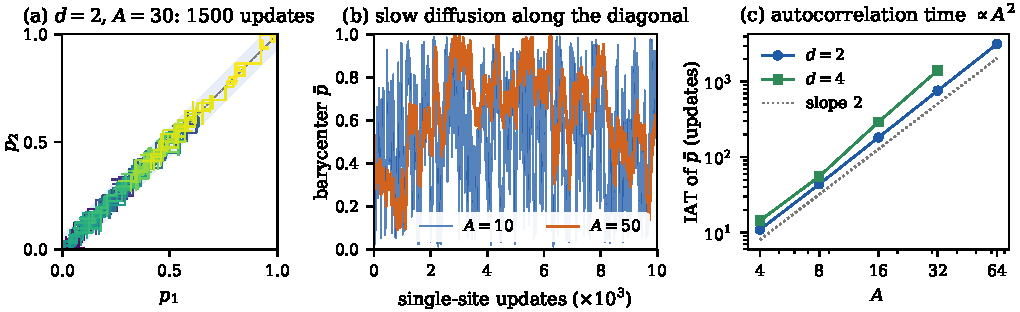
\includegraphics[width=\textwidth]{figs/fig_almost_exch.pdf}
\caption{Our simulation of the Gibbs sampler for de Finetti's prior~\eqref{eq:definetti} (complete graph, equal weights). (a)~A trajectory for $d=2$, $A=30$ from the corner $\mathbf 0$, dark to yellow over time; the band $|p_1-p_2|\le2/A$ shows it hugs the diagonal. (b)~The barycenter $\bar p$ diffuses more slowly for larger $A$. (c)~Integrated autocorrelation time of $\bar p$ in single-site updates (64 chains per point); slope 2 matches the $\Theta(dA^2)$ rate of \cref{thm:go}.}
\label{fig:ax}
\end{figure}

To see the role of the cube, remove it. Without the constraint $p\in[0,1]^d$, the target~\eqref{eq:definetti} is a degenerate Gaussian whose precision matrix $2A^2(D-C)$ is a graph Laplacian, and the sampler is a randomized Gauss--Seidel iteration for it (\cref{sec:gibbs}). The constant vector lies in the Laplacian's kernel, so along the diagonal there is no restoring force and the relaxation time is infinite; the walls cap the length of this neutral direction at order one, giving relaxation time of order $A^2$. The difficulty of the analysis lies precisely in the interaction with the boundary.

\subsection{Proof architecture}
\emph{Lower bound: concentration versus anticoncentration.} Start at the center $\frac12\mathbf 1$. A second-moment computation gives $\E[(\bar p(k)-\frac12)^2]\le 27\,k\gamma_C/(\lambda A^2)$, so after $k\ll(\lambda/\gamma_C)A^2$ steps the barycenter is still near $\frac12$. Under $\pi_{A,C}$, however, $\bar p$ is spread almost uniformly over $[0,1]$, so $\E|\bar p-\frac12|\approx\frac14$. Since $\|p-p'\|_\infty\ge|\bar p-\bar p'|$ under any coupling, the Wasserstein distance is at least about $\frac14$. This is a test-function argument: one slowly moving Lipschitz statistic certifies that the chain has not mixed.

\emph{Upper bound: a monotone, contracting coupling.} Update all copies of the chain with the same coordinate $i$ and the same uniform random number $U$, pushed through the inverse distribution function of the truncated normal. Log-concavity of the Gaussian makes this map nondecreasing in the conditional mean with slope at most one, so the coupling preserves the coordinatewise order and never increases sup-norm distances. Run four coupled copies, started at the corners $\mathbf 0$ and $\mathbf 1$, at an arbitrary state, and at stationarity. Every copy is sandwiched between the two corner copies, so once the copy from $\mathbf 0$ comes within $2\delta$ of the opposite corner, all four lie within $2\delta$ of each other, and they remain close forever. A submartingale argument for $\bar p^{\,2}$ bounds the expected time to reach the opposite corner by $O(dA^2)$, and a large-deviation estimate keeps the coordinates clustered meanwhile. Sandwiching between extremal states is the continuous cousin of the monotone coupling behind exact sampling \citep{propp1996exact}.

\subsection{Lessons}
Two lessons recur in the synthesis. First, the metric follows the structure: monotone coupling naturally controls a Wasserstein distance, and \GO\ conjecture but do not prove the same rate in total variation, since exact coupling requires bringing copies within the noise scale $O(1/A)$. Second, drift and minorization fail here for a structural reason: single-site updates from two points that differ in other coordinates have nearly singular laws, so any minorization over a macroscopic set has a tiny constant, and \GO\ report bounds exponentially bad in $A$ by that route.

%======================================================================
\section{What controls Metropolis--Hastings rates}\label{sec:mh}

Each block update in a MwG sampler is itself an MH chain targeting a conditional distribution, so the local factor in~\eqref{eq:principle} is a question about MH convergence. \BJ\ review this subject; we extract the lessons that matter here.

\subsection{The independence sampler: a solvable case}
If the proposal ignores the current state, $q(x,y)=q(y)$, and the importance weight $w=\pi/q$ is bounded by $M$, then for every $x$,
\[
P(x,dy)\;\ge\;q(y)\min\Bigl\{1,\frac{w(y)}{w(x)}\Bigr\}dy\;\ge\;q(y)\,\frac{w(y)}{M}\,dy=\frac{\pi(dy)}{M}.
\]
This is a minorization over the whole space, so a coupling that regenerates with probability $1/M$ per step gives $\|P^t(x,\cdot)-\pi\|_\TV\le(1-1/M)^t$: the chain is uniformly ergodic \citep{tierney1994,mengersen1996}. The rate $1-1/M$ is exact \citep{wang2022exact}; if $w$ is unbounded the chain is not even geometrically ergodic \citep{mengersen1996}, and \BJ\ stress that subgeometric convergence is common for heavy-tailed targets. The catch is dimension: for a standard Gaussian target in $\mathbb R^d$, a Gaussian proposal with standard deviation $\sigma>1$ has $M=\sigma^d$, exponential in $d$ (and $\sigma<1$ makes $w$ unbounded). An independence sampler is hopeless for a large joint update but excellent for a small block, a fact \ARZ\ exploit (\cref{sec:arz}).

\subsection{Random-walk Metropolis: from qualitative to quantitative}
For random-walk proposals $N(x,hI)$, classical theory characterizes geometric ergodicity through tail behavior \citep{mengersen1996,roberts1996geometric,jarner2000}. Quantitative rates are much harder, and \BJ\ note that explicit rates for MH in practical problems are rare. The most complete results assume strong log-concavity: if the curvature of $-\log\pi$ lies between $m$ and $L$, random-walk Metropolis with step size $h\asymp1/(Ld)$ has spectral gap of order $m/(Ld)$ \citep{andrieu2024explicit}, recovering the $1/d$ scaling predicted by \citet{roberts1997weak}.

\subsection{Lower bounds: to leave, you must accept}
The simplest lower bound is also one of the most useful. Let $\bar\alpha(x)=\int\alpha(x,y)\,q(x,y)\,dy$ be the probability of accepting a move from $x$. Staying put for $t$ steps has probability at least $(1-\bar\alpha(x))^t$, and $\pi$ puts no mass on the single point $x$, so for any geometric rate $\rho$ \citep{brown2024lower},
\begin{equation}\label{eq:bjlower}
\|P^t(x,\cdot)-\pi\|_\TV\ge\bigl(1-\bar\alpha(x)\bigr)^t\ \ \text{for all }t,\qquad\text{hence}\qquad\rho\ge1-\inf_x\bar\alpha(x).
\end{equation}
The power lies in bounding $\bar\alpha(x)$. For MH, $\bar\alpha(x)=\int\min\{q(x,y),\,\pi(y)q(y,x)/\pi(x)\}\,dy\le\sup q/\pi(x)$, so a Gaussian proposal $N(\mu(x),hS)$, which covers random-walk Metropolis and MALA, has
\[
\bar\alpha(x)\le\frac{1}{\pi(x)\,(2\pi h)^{d/2}\det(S)^{1/2}}.
\]
Two consequences follow. If $-\log\pi$ is strongly convex with curvature at least $1/\xi$, random-walk Metropolis has $\bar\alpha(x^*)\le(1+h/\xi)^{-d/2}$ at the mode $x^*$, so a fixed step size drives $\rho\to1$ exponentially fast in $d$, and $h\lesssim1/d$ is forced, as optimal scaling predicts but under much weaker assumptions. If $\pi$ is a posterior concentrating at rate $n^{-1/2}$, then $\pi(x^*)\gtrsim n^{d/2}$ and $\bar\alpha(x^*)\lesssim(nh)^{-d/2}$ up to constants, so the step size must shrink like $1/n$ as data accumulate. Hence the moral drawn by \BJ: tuning must depend on \emph{both} the dimension and the sample size. Since leaving a small set requires an acceptance, the same quantity also bounds conductance from above.

\subsection{Consequences for local updates}
All of this applies to a block update with target $\pi_i(\cdot\mid x_{-i})$, with the block dimension $d_i$ and the conditional curvature in place of $d$ and the global one. Using these tools, \ARZ\ bound the conditional conductance (\cref{sec:arz}) of two common block updates when the conditional log-density has curvature between $m_i$ and $L_i$: an independence proposal centered at the conditional mode achieves at least $(L_i/m_i)^{-d_i/2}$, exponentially small in the block dimension, while random-walk Metropolis with $h_i\asymp1/(d_iL_i)$ achieves order $(d_iL_i/m_i)^{-1/2}$, only polynomially small. Neither bound involves the total dimension $d$, which is what makes dimension-free MwG possible.

%======================================================================
\needspace{14\baselineskip}
\section{Metropolis-within-Gibbs: inheriting the speed of the ideal sampler}\label{sec:mwg}

\subsection{Two blocks: a qualitative map}\label{sec:qjmap}
\begin{wrapfigure}{r}{0.36\textwidth}
\vspace{-14pt}
\centering
\begin{tikzpicture}[node distance=1.15cm and 1.9cm, every node/.style={font=\small},
  s/.style={draw=black!60, circle, minimum size=0.92cm, inner sep=0pt},
  imp/.style={-{Stealth[length=2.1mm]}, thick},
  cond/.style={-{Stealth[length=2.1mm]}, thick, dashed, black!55}]
\node[s,fill=blue!6] (DG) {DG};
\node[s,fill=blue!6,right=of DG] (RG) {RG};
\node[s,fill=orange!10,below=of DG] (DC) {DC};
\node[s,fill=orange!10,below=of RG] (RC) {RC};
\draw[imp] (DG.12) -- (RG.168);
\draw[imp] (RG.192) -- (DG.348);
\draw[imp] (DC.78) -- (DG.282);
\draw[cond] (DG.258) -- (DC.102);
\draw[imp] (RC.78) -- (RG.282);
\draw[cond] (RG.258) -- (RC.102);
\draw[imp] (DC.12) -- (RC.168);
\draw[cond] (RC.192) -- (DC.348);
\end{tikzpicture}
\caption{Implications between geometric ergodicity of two-block samplers (after \QJ). Solid: always; dashed: under the covering condition of \cref{prop:qjmap}(c).}
\label{fig:qjmap}
\vspace{-10pt}
\end{wrapfigure}
\QJ\ replace the $X$-update of DG or RG by an MH step with proposal $q(\cdot\mid x,y)$, giving deterministic-scan (DC) and random-scan (RC) conditional Metropolis--Hastings samplers, and ask: if one of the four samplers is geometrically ergodic, which others must be (\cref{fig:qjmap})?

\begin{proposition}[\QJ]\label{prop:qjmap}
(a) For every proposal, $\rho(P_\RC)\ge\bar\gamma$; hence if RC or DC is geometrically ergodic for some proposal, so are both Gibbs samplers. (b) If DC is geometrically ergodic, so is RC with the same proposal. (c) If the proposal covers the conditional, $\sup_{x',x,y}\pi_{X\mid Y}(x'\mid y)/q(x'\mid x,y)\le C<\infty$, then geometric ergodicity of DG (resp.\ RG) implies that of DC (resp.\ RC). (d) Without such a condition, RC can be geometrically ergodic while DC is not.
\end{proposition}

Part (a) has a one-line proof worth seeing, because it explains why no MH tuning can rescue a bad Gibbs sampler. Take mean-zero, unit-variance $g(x)$ and $h(y)$. In one RC step, with probability $r$ the MH move changes only $x$ and leaves $h(Y)$ untouched; with probability $1-r$ we redraw $Y$ given $X$, replacing $h(Y)$ by $\E[h(Y)\mid X]$. Either way the correlation with $g(X)$ is preserved, so $\langle P_\RC h,g\rangle_\Pi=\mathrm{Corr}(g(X),h(Y))$, and the supremum over $g,h$ gives $\|P_\RC\|\ge\bar\gamma$: dependence between the blocks is a barrier that local updates cannot remove. Parts (b) and (c) rest on a comparison lemma: if $P_1(x,\cdot)\ge\delta P_2(x,\cdot)$ for all $x$, both kernels are $\pi$-invariant, and $\|P_2\|<1$, then $P_1=\delta P_2+(1-\delta)R$ with $R$ a $\pi$-invariant kernel, so $\|P_1\|\le\delta\|P_2\|+1-\delta<1$. Under the covering condition the MH step dominates $C^{-1}$ times the exact draw, as for the independence sampler in \cref{sec:mh}, so $P_\RC\ge C^{-1}P_\RG$ \citep{jones2014conditional}; (b) uses $P_\RC^4\ge r^2(1-r)^2P_\DC^2$, and (d) is a periodic two-point example. When \emph{both} blocks use MH, whether geometric ergodicity of the deterministic-scan version implies that of the others is open.

\subsection{A first quantitative comparison, and its limits}
For random scans, the comparison method of \cref{sec:history} gives a quantitative version at once. Suppose each conditional MH kernel, viewed as a chain on block $i$ with $x_{-i}$ frozen, has spectral gap at least $\kappa_{\mathrm{gap}}$ for every $x_{-i}$. Then the Dirichlet form of the $i$th MwG update is at least $\kappa_{\mathrm{gap}}$ times $\E[\mathrm{Var}(f\mid X_{-i})]$, the Dirichlet form of the exact update (\cref{sec:operator}). Averaging over $i$,
\begin{equation}\label{eq:gapcomp}
\Gap(P_{\mathrm{MwG}})\;\ge\;\kappa_{\mathrm{gap}}\cdot\Gap(G),
\end{equation}
and \citet{qin2025spectral} sharpen such bounds under weaker assumptions. The difficulty is the word \emph{every}. In a hierarchical model, a random-walk update for a group parameter $\theta_j$ works well for typical hyperparameters $\psi$, but as $\psi$ moves into its tails the conditional law of $\theta_j$ becomes far narrower or wider than the proposal and the conditional gap tends to zero. Then $\kappa_{\mathrm{gap}}=0$ and~\eqref{eq:gapcomp} is vacuous, even though such regions have negligible posterior probability.

\subsection{Conditional conductance}\label{sec:arz}
\ARZ\ resolve this by moving from spectral gaps to $s$-conductance, which can ignore sets of small probability. For a random-scan kernel $P=\frac1d\sum_iP_i$, where $P_i$ updates block $i$ with a $\pi_i(\cdot\mid x_{-i})$-invariant kernel $P_i^{x_{-i}}$, define the \emph{conditional conductance} of a block update and its worst case over a set $K\subseteq\X$:
\[
\kappa\bigl(P_i^{x_{-i}}\bigr)=\inf_{B}\frac{\int_BP_i^{x_{-i}}(x_i,B^c)\,\pi_i(dx_i\mid x_{-i})}{\pi_i(B\mid x_{-i})\,\pi_i(B^c\mid x_{-i})},\qquad\kappa(P,K)=\min_i\ \inf_{x\in K}\ \kappa\bigl(P_i^{x_{-i}}\bigr).
\]
The normalization makes an exact draw have conditional conductance exactly $1$, because from $B$ it lands in $B^c$ with probability $\pi_i(B^c\mid x_{-i})$, so its flow out of $B$ is $\pi_i(B)\pi_i(B^c)$. Thus $\kappa$ measures how close a local update is to exact sampling.

\begin{theorem}[\ARZ]\label{thm:arz}
Let $G$ be the random-scan Gibbs kernel. For all $s\in[0,\frac12)$, $\Phi_s(P)\ge\kappa(P,\X)\,\Phi_s(G)$. If, in addition, every conditional kernel is reversible and positive semi-definite, then for every $K\subseteq\X$,
\[
\kappa(P,K)\,\Phi_s(G)-\frac{\pi(K^c)}{s}\;\le\;\Phi_s(P)\;\le\;\Phi_s(G).
\]
\end{theorem}

\emph{Proof idea (for $K=\X$).} Fix a set $A$ and a block $i$. Freezing $x_{-i}$ cuts $A$ into a slice $A_i(x_{-i})=\{x_i:x\in A\}$. The exact update's flow out of the slice is $\pi_i(A_i)\pi_i(A_i^c)$, and by definition the MH update's flow is at least $\kappa(P_i^{x_{-i}})$ times that. Integrating over $x_{-i}$ gives $P_i(\partial A)\ge\kappa\,G_i(\partial A)$; averaging over $i$ and dividing by $\pi(A)$ gives the first inequality. The comparison is \emph{fiberwise}: it never asks how the blocks interact, only how each local move compares with an exact draw on each slice. Restricting to $K$ loses at most the flow out of $A\cap K^c$, producing the $\pi(K^c)/s$ term, and positive semi-definiteness ensures a local move never leaks more than an exact draw. The lower bound is tight: the lazy kernel that makes an exact draw with probability $c$ and otherwise stays put has $\kappa=c$ and $\Phi_s(P)=c\,\Phi_s(G)$.

With~\eqref{eq:sconductance} and $s=\varepsilon/(2M)$, \cref{thm:arz} gives, from an $M$-warm start,
\[
\tmix(P;\varepsilon,M)\;\lesssim\;\frac{\log(2M/\varepsilon)}{\kappa(P,K)^2\,\Phi_s(G)^2}\qquad\text{whenever }\ \pi(K^c)\ll s\,\kappa(P,K)\,\Phi_s(G).
\]
The slowdown relative to Gibbs depends on the number of blocks only through the minimum defining $\kappa$, so if every block update is reasonably good, MwG is slower than exact Gibbs by a factor that does not grow with the dimension; the square, inherited from Cheeger's inequality, is the price of working with conductance.

\subsection{Dimension-free MwG for hierarchical models}\label{sec:hier}
The flagship application is the two-level hierarchical model
\[
Y_j\mid\theta_j\sim f(\cdot\mid\theta_j),\qquad\theta_j\mid\psi\overset{\text{iid}}{\sim}p(\cdot\mid\psi),\qquad\psi\sim p_0,\qquad j=1,\dots,J,
\]
for example a hierarchical logistic regression with $J$ groups. Given $\psi$ the local parameters are conditionally independent, so the $\theta$-update splits into $J$ small independent updates of cost $O(1)$ each, while $\psi$ is low-dimensional. \ARZ\ study the regime $J\to\infty$ with data generated from the model, so that both the numbers of parameters and observations grow, and assemble three ingredients.
\begin{enumerate}[leftmargin=1.4em,nosep]
\item \emph{Local factor.} The $\theta$-update is a product of $J$ independent kernels; the gap of a product is the minimum gap, so Cheeger's inequality gives conditional conductance at least $\min_j\kappa_j^2/4$, independent of $J$. Each $\theta_j$-update need only be good for $\psi$ near the true value $\psi^*$.
\item \emph{Ignoring bad regions.} By the Bernstein--von Mises theorem the posterior of $\psi$ concentrates near $\psi^*$, so taking $K=\{\psi\text{ near }\psi^*\}$ makes the penalty $\pi(K^c)/s$ vanish as $J\to\infty$.
\item \emph{Global factor.} The exact Gibbs sampler has $s$-conductance bounded away from zero with probability tending to one \citep{ascolani2024dimension}, using that $\psi$ depends on $\theta$ only through a low-dimensional sufficient statistic, plus a perturbation bound: if $\|\pi_1-\pi_2\|_\TV\le\delta$, the corresponding Gibbs samplers satisfy $\Phi_s(G_1)\ge\Phi_{s-\delta}(G_2)-4\delta/s$.
\end{enumerate}
The conclusion is that $\tmix(P_J;\varepsilon,M)=O_P(1)$ as $J\to\infty$: the number of iterations is bounded in probability, so the total cost is $O(J)$ from a warm start and $O(J\log J)$ from an explicit start that \ARZ\ construct. Gradient-based methods (MALA, Hamiltonian Monte Carlo) also pay $O(J)$ per iteration but need a growing number of iterations; in \ARZ's experiments their autocorrelation times grow with $J$ while those of Gibbs and MwG stay flat.

The perturbation bound shows why $s>0$ is essential. Exact conductance is sensitive to sets of arbitrarily small probability: restricting a standard bivariate Gaussian to $\{x,y\le n\}\cup\{x,y\ge n\}$ changes it by a vanishing amount in total variation as $n\to\infty$, yet the Gibbs sampler can no longer cross between the two pieces, so its conductance drops from $1$ to $0$ (\ARZ). Approximate conductance is the right currency for combining MCMC analysis with statistical asymptotics, which control distributions only up to small total-variation errors.

\subsection{Limits of the comparison}
The fiberwise argument relies on the random scan. For a deterministic scan a naive version multiplies the conditional conductances of all $d$ blocks, a factor exponentially small in $d$; tight bounds for deterministic-scan MwG, widely used in practice, remain open (\ARZ). The bounds also expose a blocking trade-off: larger blocks weaken the dependence between blocks, improving $\Phi_s(G)$, but lower the conditional conductance, exponentially in the block dimension for independence proposals and polynomially for random walks (\cref{sec:mh}).

%======================================================================
\section{Synthesis: what the four papers say together}\label{sec:synthesis}

\subsection{One principle, three currencies}
Placed side by side, \QJ\ and \ARZ\ prove the same principle in different currencies, while \GO\ and \BJ\ study the two factors it combines. In the $L^2$ currency for two blocks, \QJ\ show that a good Gibbs sampler is \emph{necessary} for a good hybrid ($\rho(P_\RC)\ge\bar\gamma$) and, with a uniformly good local update, \emph{sufficient}. Comparison of Dirichlet forms gives the spectral-gap version~\eqref{eq:gapcomp}, and \ARZ\ prove the two-sided conductance version (\cref{thm:arz}), robust enough to survive high dimension. The upper inequalities say MwG is never faster than the Gibbs sampler it imitates; the lower ones say it is slower by at most the local quality factor. Each currency has a price: the $L^2$ results are exact but limited to two blocks or uniform conditions, while conductance handles many blocks and bad regions but loses a square and needs warm starts.

The principle yields a practical diagnostic that \ARZ\ and \BJ\ both point toward: a slow MwG sampler is slow either because the Gibbs sampler it imitates is slow or because its local moves are poor, and the remedies differ. Strong dependence between blocks calls for reparameterization, blocking, or collapsing \citep{roberts1997updating,papaspiliopoulos2007general}; poor local moves call for step sizes matched to the conditional scale, as \BJ's lower bounds demand, or for several MH steps per block, which raises $\kappa$. The principle also licenses transferring decades of work on improving Gibbs samplers to their hybrid versions.

\subsection{The geometry of slow mixing}
Our Gibbs examples share one geometry. In the bivariate Gaussian the ridge has width $\sqrt{1-\rho^2}$ and the rate is governed by $\bar\gamma=|\rho|$; in \GO's model the ridge is the cube's diagonal, with width $1/A$ and mixing time $\Theta(A^2)$; in hierarchical models a ridge appears in the centered parameterization when data are weakly informative, and \ARZ's centered versus non-centered comparison shows the same effect for MwG. In each case an axis-aligned sampler is slow exactly when the mass lies along a thin set not aligned with the blocks, with slowdown like the squared aspect ratio. The tools differ (maximal correlation, Gauss--Seidel spectra, diffusion and coupling), but all measure how far $\pi$ is from a product across the blocks.

\subsection{Concentration helps and hurts}
\GO\ let $A\to\infty$, \ARZ\ let $J\to\infty$, and \BJ\ let $d$ and $n$ grow; across these regimes concentration plays opposite roles. In \GO, concentration onto the diagonal \emph{hurts}, because it creates a ridge misaligned with the coordinate moves. In \BJ, posterior concentration hurts a random-walk sampler unless its step size shrinks with $n$, because a fixed proposal overshoots the shrinking bulk. In \ARZ, posterior concentration of $\psi$ \emph{helps}: it drives the Gibbs sampler toward a well-conditioned limit and confines the chain to where local updates are good. A unifying reading is that exact Gibbs moves are \emph{locally self-tuning}, since a conditional draw adapts automatically to the conditional width ($1/A$ in \GO), but cannot repair \emph{global} misalignment; Metropolis moves must be tuned locally, but a well-tuned MwG sampler then inherits whatever global behavior its Gibbs sampler has. Concentration helps when it is aligned with the block structure and hurts when it is not.

\subsection{What does it mean to know a rate?}
The papers also span the range of available guarantees (\cref{tab:compare}): an exact identity between two rates but not the rates themselves (\QJ); matching upper and lower bounds, the gold standard, for one model in one metric (\GO); dimension-free upper bounds that are asymptotic and from warm starts (\ARZ); and lower bounds, which cannot show an algorithm is fast but can show it is slow (\BJ). Explicit, two-sided, total-variation bounds for realistic hybrid samplers remain out of reach.

\begin{table}[t]
\centering\footnotesize
\renewcommand{\arraystretch}{1.18}
\begin{tabularx}{\textwidth}{@{}L{1.6cm}YYYY@{}}
\toprule
 & \textbf{Qin \& Jones (2022)} & \textbf{Ascolani et al.\ (2026)} & \textbf{Gerencs\'er \& Ottolini (2023)} & \textbf{Brown \& Jones (2024a)} \\
\midrule
Question & Does scan order, or an MH substitute, change the rate? & When does MwG scale as well as Gibbs? & How long must de Finetti's Gibbs sampler run? & What controls MH rates; when must MH fail? \\
Samplers & two-block DG, RG, DC, RC & random-scan coordinate-wise (MwG) & random-scan Gibbs, truncated normals & independence, random walk, MALA \\
Currency & $L^2$ rate; geometric ergodicity & $s$-conductance; TV from warm start & Wasserstein (sup-norm cost) & TV, $L^2$, Wasserstein \\
Main tools & two projections; kernel minorization comparison & conditional conductance; perturbation; Bernstein--von Mises & monotone coupling; martingales; anticoncentration & drift \& minorization; spectral; holding probability \\
Regime & fixed target, any two blocks & $J\to\infty$, random data & fixed $d$ and graph, $A\to\infty$ & $d,n\to\infty$ \\
Guarantee & exact identity; qualitative implications & $\tmix=O_P(1)$, cost $O(J)$ & matching $\Theta(A^2)$ bounds & exact (independence); lower bounds \\
Key insight & maximal correlation is a barrier no MH update can beat & slowdown $=$ local quality, independent of $d$ & diffusion along a ridge; squared aspect ratio & to leave, MH must accept; tune with $d$ and $n$ \\
\bottomrule
\end{tabularx}
\caption{The four papers side by side.}
\label{tab:compare}
\end{table}

%======================================================================
\section{Open problems}\label{sec:open}
\begin{itemize}[leftmargin=1.3em,itemsep=2pt]
\item \emph{Deterministic scans.} \QJ\ (beyond two blocks) and \ARZ\ (for MwG) both single out deterministic scans as the main gap. The obstacle is non-reversibility: products of more than two projections have no planar picture, and fiberwise flow comparisons multiply across blocks.
\item \emph{Fully hybrid samplers.} For two blocks both updated by MH, whether geometric ergodicity of the deterministic-scan version implies that of the others is open (\QJ).
\item \emph{Total variation and sharp graph dependence.} \GO\ conjecture $\Theta(A^2)$ in total variation; their bounds differ by $d^3$ for the cycle; the posterior case and the limit $d\to\infty$ (a low-temperature interacting particle system) are open.
\item \emph{Explicit guarantees.} \ARZ's results are asymptotic and mostly from warm starts; explicit constants would turn them into usable stopping rules.
\item \emph{Lower bounds for hybrids.} Holding-probability lower bounds should extend to MwG and Hamiltonian Monte Carlo (\BJ); a lower-bound counterpart of \cref{thm:arz} would show when MwG is provably slow.
\item \emph{Multimodality.} The decomposition principle does not help when the Gibbs sampler itself is slow because of separated modes; there, tools such as decomposition across modes \citep{madras2002} are needed.
\end{itemize}

%======================================================================
\section{Conclusion}\label{sec:conclusion}
Correctness of MCMC is a local property; speed is a global one. The exact Gibbs sampler is an idealized algorithm whose speed is set by the geometry of the target, measured by maximal correlation, Gauss--Seidel spectra, or, as \GO\ show for de Finetti's prior, diffusion along a ridge. Metropolis-within-Gibbs replaces each exact projection by a Metropolis--Hastings chain, and its speed is the Gibbs speed degraded by the quality of these local chains: exactly so in the two-block geometry of \QJ, and quantitatively, even as dimension grows, in the conductance framework of \ARZ; \BJ\ explain what controls that local quality and, through lower bounds, when it collapses. For practice, the lesson is to diagnose a slow sampler with two separate questions: is the ideal sampler slow, and are the local moves poor? For theory, it is that choosing the right currency, an $L^2$ norm, a conductance, or a Wasserstein distance, is often what makes a convergence proof possible.

\section*{References}
\renewcommand{\bibsection}{}
\setlength{\columnsep}{18pt}
\begin{multicols}{2}
\bibliographystyle{abbrvnat}
\bibliography{refs}
\end{multicols}

\end{document}
